%
% fig-kurve.tex
%
% (c) 2024 Prof Dr Andreas Müller
%
\begin{figure}
\centering
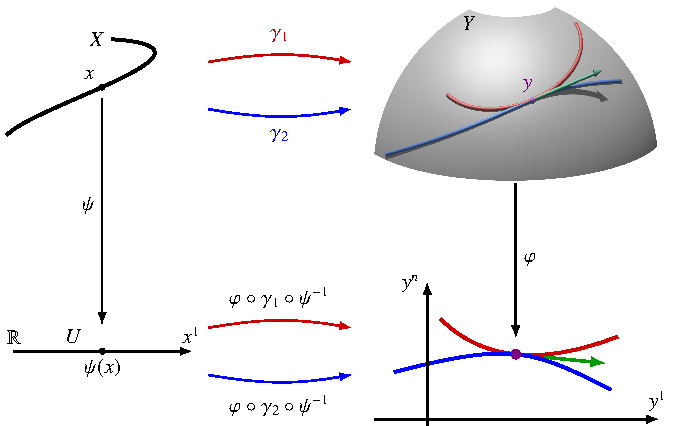
\includegraphics{chapters/020-koordinaten/images/kurve.pdf}
\caption{Die Kurven $\gamma_1$ und $\gamma_2$ sind tangential im
Punkt $y$, wenn $\gamma_1(x)=y=\gamma_2(x)$ und ausserdem die
Ableitungen der Zusammensetzungen $\varphi\circ\gamma_i\circ\psi^{-1}$
in $\psi(x)$ übereinstimmen.
Es ist nicht sinnvoll, von einem Tangentialvektor ``in $Y$'' (grün,
oben rechts) zu sprechen, erst durch das Koordinatensystem kann
das Konzept des Tangentialvektors konsistent definiert werden.
\label{buch:koordinaten:tangentialvektoren:fig:kurve}}
\end{figure}
